\documentclass[12pt]{article}

\usepackage{amsmath}    % need for subequations
\usepackage{graphicx}   % need for figures
\usepackage{verbatim}   % useful for program listings
\usepackage{color}      % use if color is used in text
\usepackage{subfigure}  % use for side-by-side figures
\usepackage{hyperref}   % use for hypertext links, including those to external documents and URLs


\usepackage{graphicx}
\graphicspath{ {./images/} }

\setlength{\baselineskip}{15.0pt}    % 16 pt usual spacing between lines

\setlength{\parskip}{3pt plus 2pt}
\setlength{\parindent}{20pt}
\setlength{\oddsidemargin}{0.5cm}
\setlength{\evensidemargin}{0.5cm}
\setlength{\marginparsep}{0.75cm}
\setlength{\marginparwidth}{2.5cm}
\setlength{\marginparpush}{1.0cm}
\setlength{\textwidth}{150mm}

\begin{comment}
\pagestyle{empty} % doesn't count for page numbers
\end{comment}


\begin{document}

    \begin{titlepage}
        \begin{center}
            {\LARGE A Mathematical Modelling of the \\ Falcon 9 Hover Slam}
            \break
            \\
            {\large A Mathematical Exploration}
            \break
            %\small{Written by Johan-Petter R. Dragic}
           % \date{06.11.2018}
            

                % ADD BREAK HERE
            \vspace{14mm}
            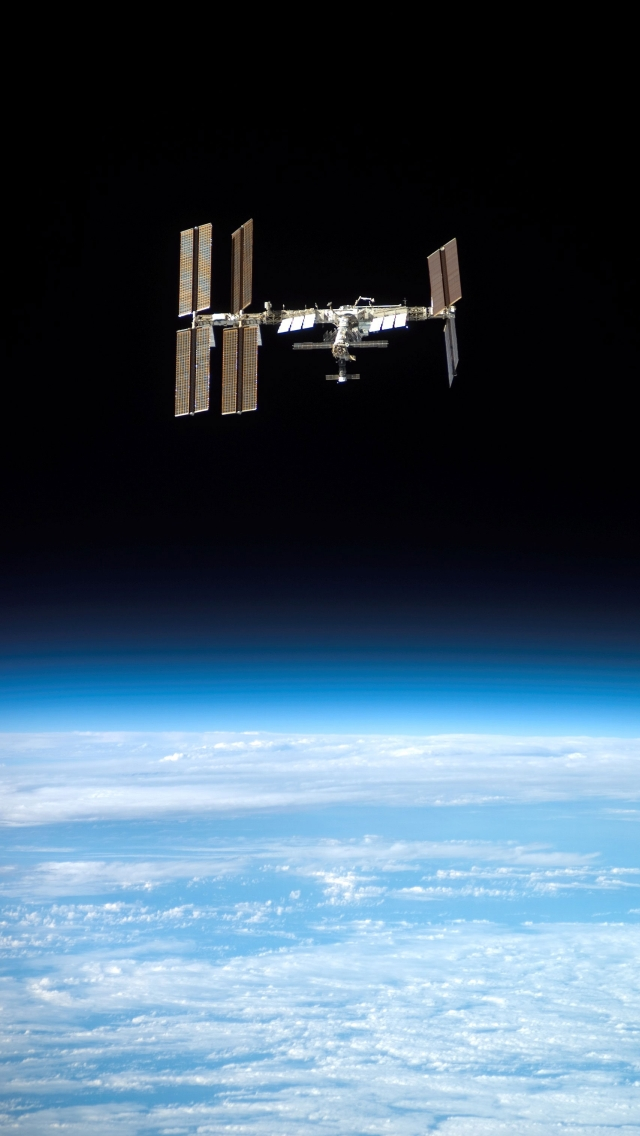
\includegraphics[scale=1.5]{iss2.jpg}
            % source pic2: https://gisgeography.com/polar-orbit-sun-synchronous-orbit/
            

        \end{center}
    \end{titlepage}

    \tableofcontents
    \thispagestyle{empty}
    \newpage
    
 
    \addtocounter{page}{-1}
    \section{Introduction} % and personal engagement
    The International Space Station (commonly referred to as the ISS) is a man-made, habitable satellite developed in a joint venture among five agencies: NASA (USA), 
    Rocosmos (Russia), JAXA (Japan), The European Space Agency, and the Canadian space agency. The first module was launched on the Russian "Proton" rocket in 1998, 
    and the last module to be launched was the "International Docking Adatper-2", launched by the private company- SpaceX in July 2016.





        


        \subsection{Personal engagement}



    \section{Background theory}
        \subsection{What are orbits}
    \section{Modelling}

    

\end{document}

